
%\addcontentsline{toc}{chapter}{Anhang}
\cftaddtitleline{toc}{chapter}{Anhang}{}
\pagenumbering{Roman}
\appendix


%\chapter{Ausschreibung Bachelorarbeit}\label{anhang_ausschreibung}
% 
%\includepdf{../ressources/Projektorganisation/Ausschreibung.pdf}
%
%
%\chapter{Projektplanung}  \label{anhang_projektplan} 
%%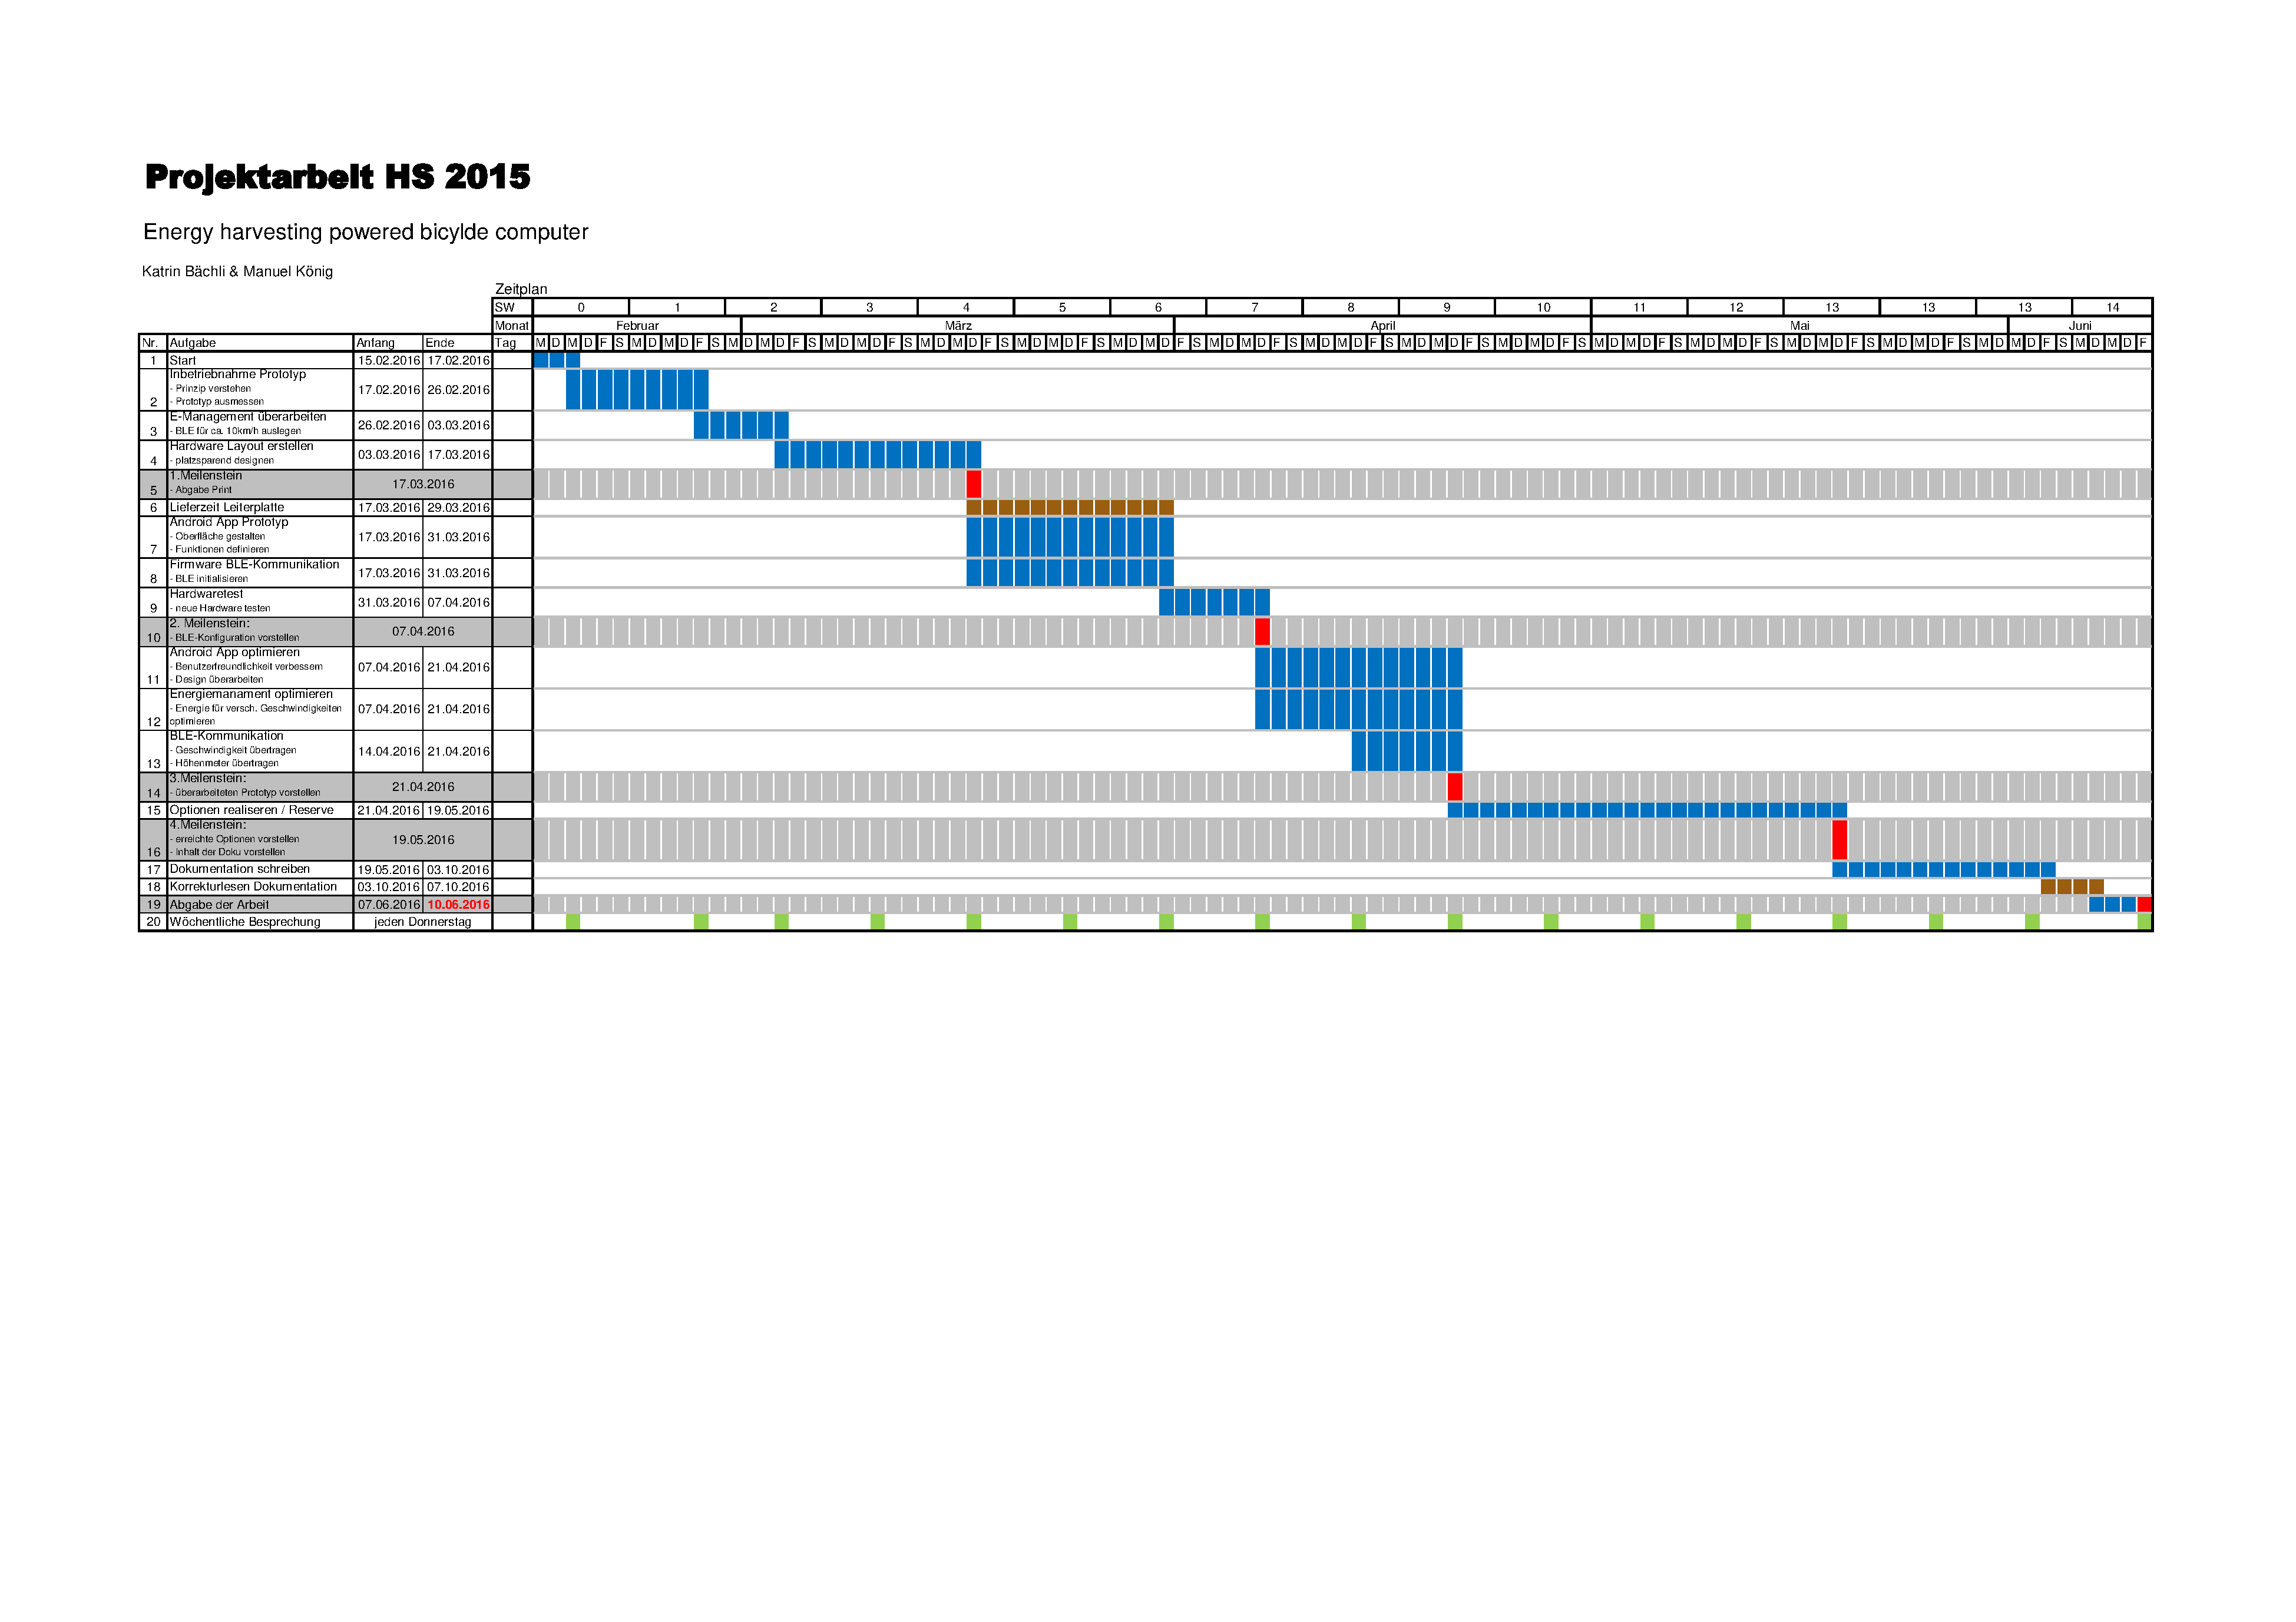
\includepdf [landscape = true, pages=-] {../ressources/Projektorganisation/PlannungV0.pdf}
%
%\vspace*{\fill}\par
%\pagebreak

%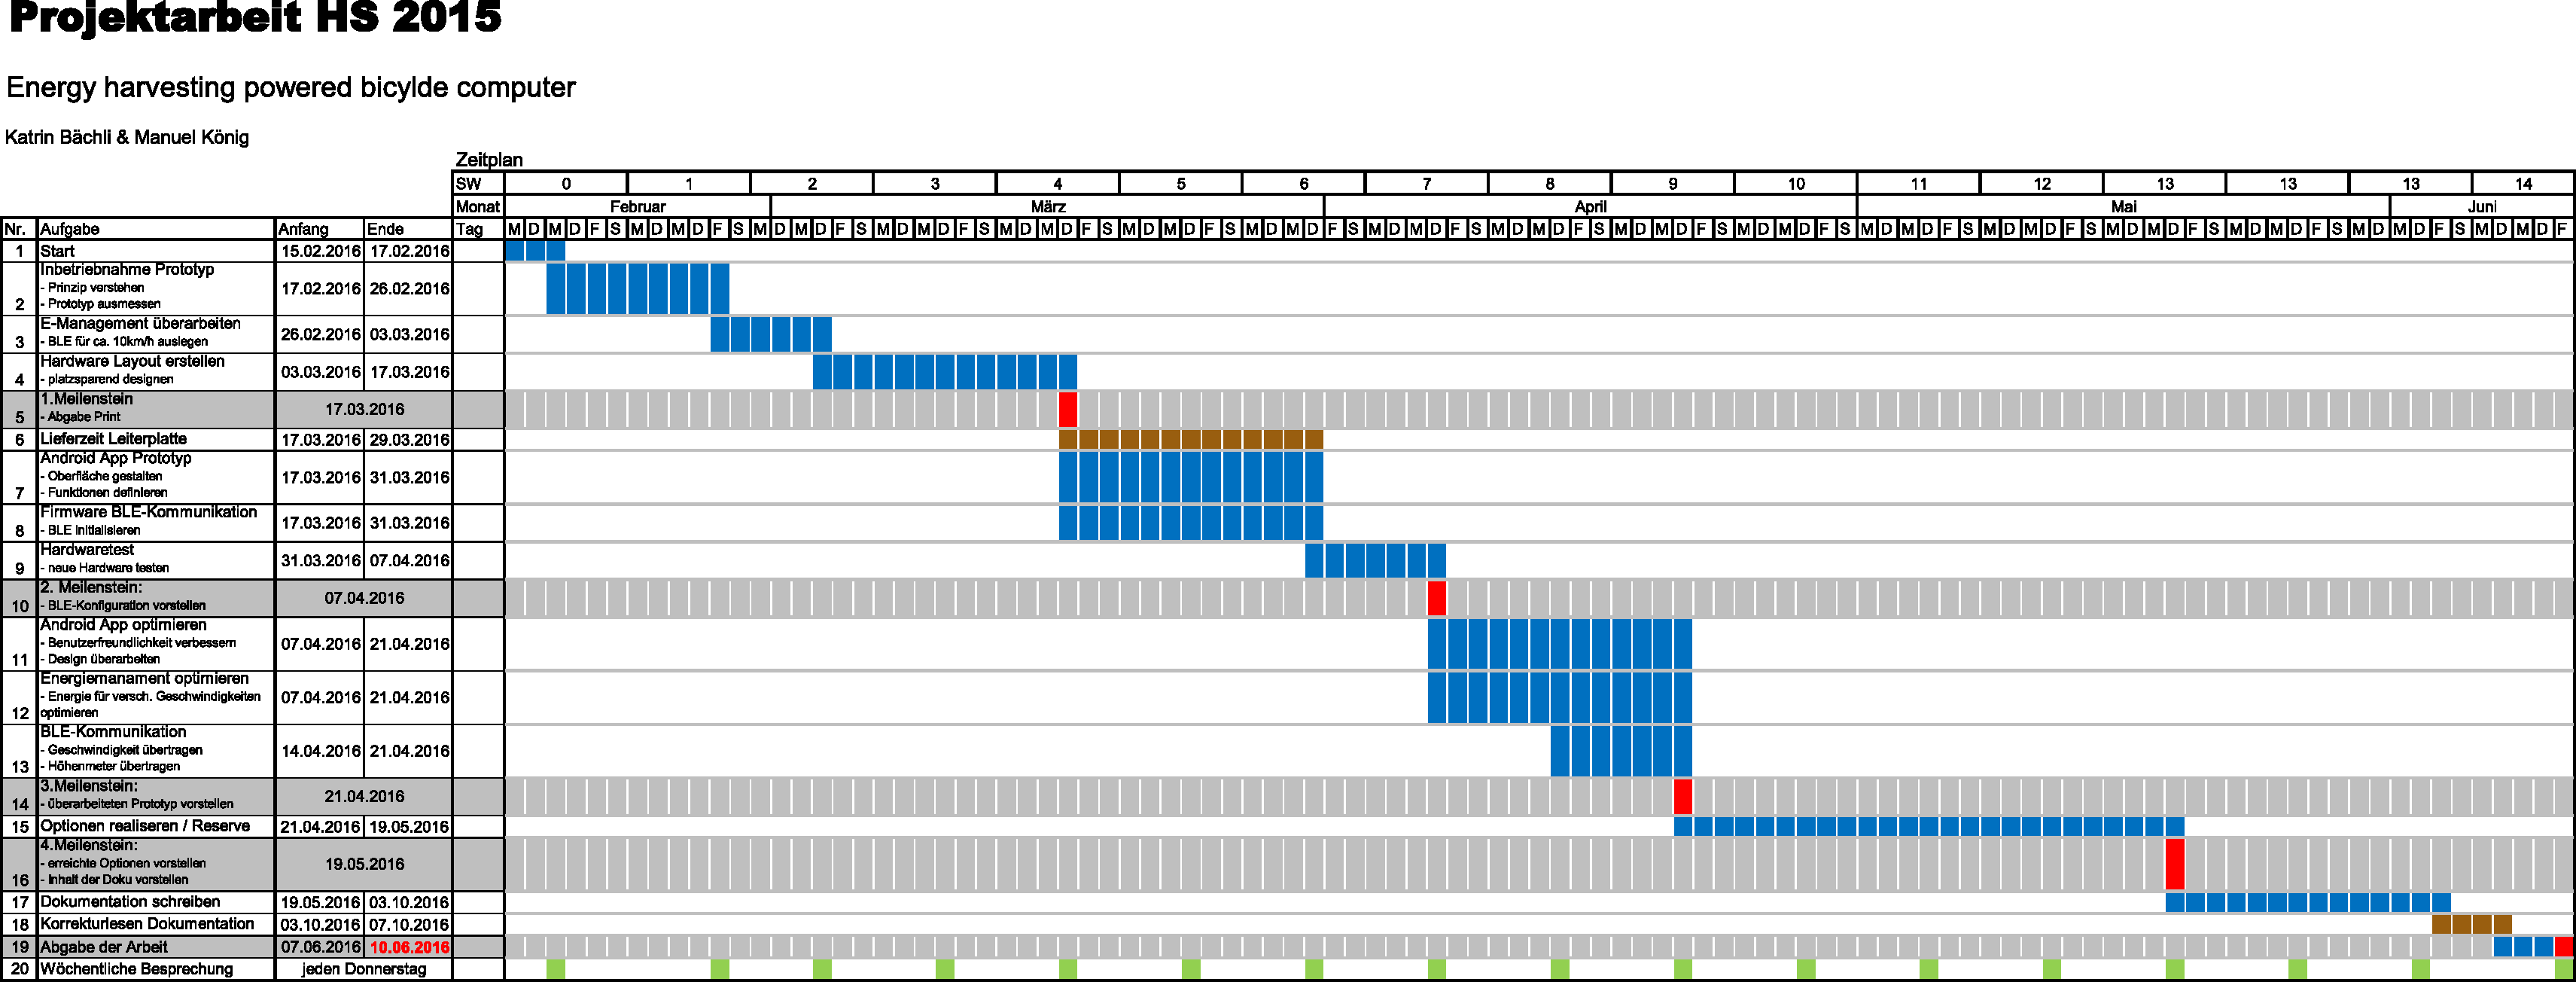
\includegraphics[width=\textheight ,angle=90,origin=c]{../ressources/Projektorganisation/PlannungV0-cropped.pdf}

\chapter{Ausschreibung Bachelorarbeit}

\begin{figure}[h]
    \includegraphics {7Anhang/docs/Ausschreibung.pdf} 
     \caption{Offizielle Ausschreibung der Arbeit}\label{Ausschreibung} 
\end{figure}



\chapter{Blockdiagramm EM8500}\label{anhang_em8500} 
\begin{figure}[h]
    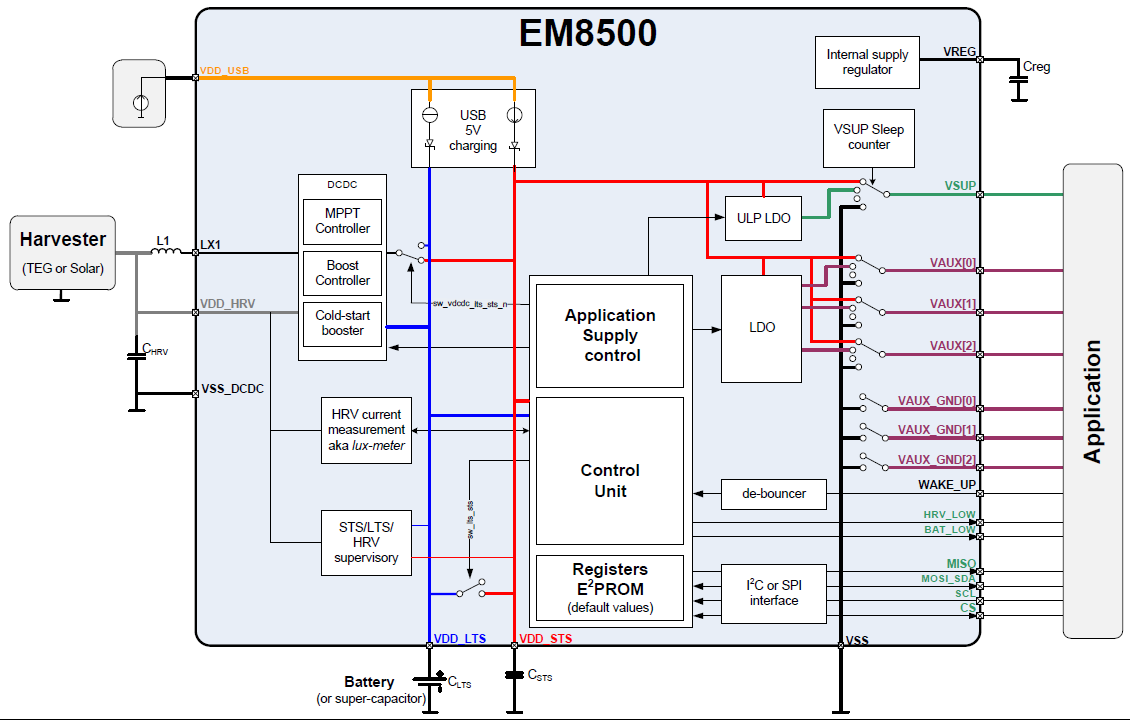
\includegraphics {7Anhang/imag/blockdiagrammEm8500.png} 
     \caption{Blockschema Sensortag}
\end{figure}



\chapter{Funktionsblöcke Sensortag von Texas Instrument}\label{anhang_sensortag} 



\begin{figure}[h]
    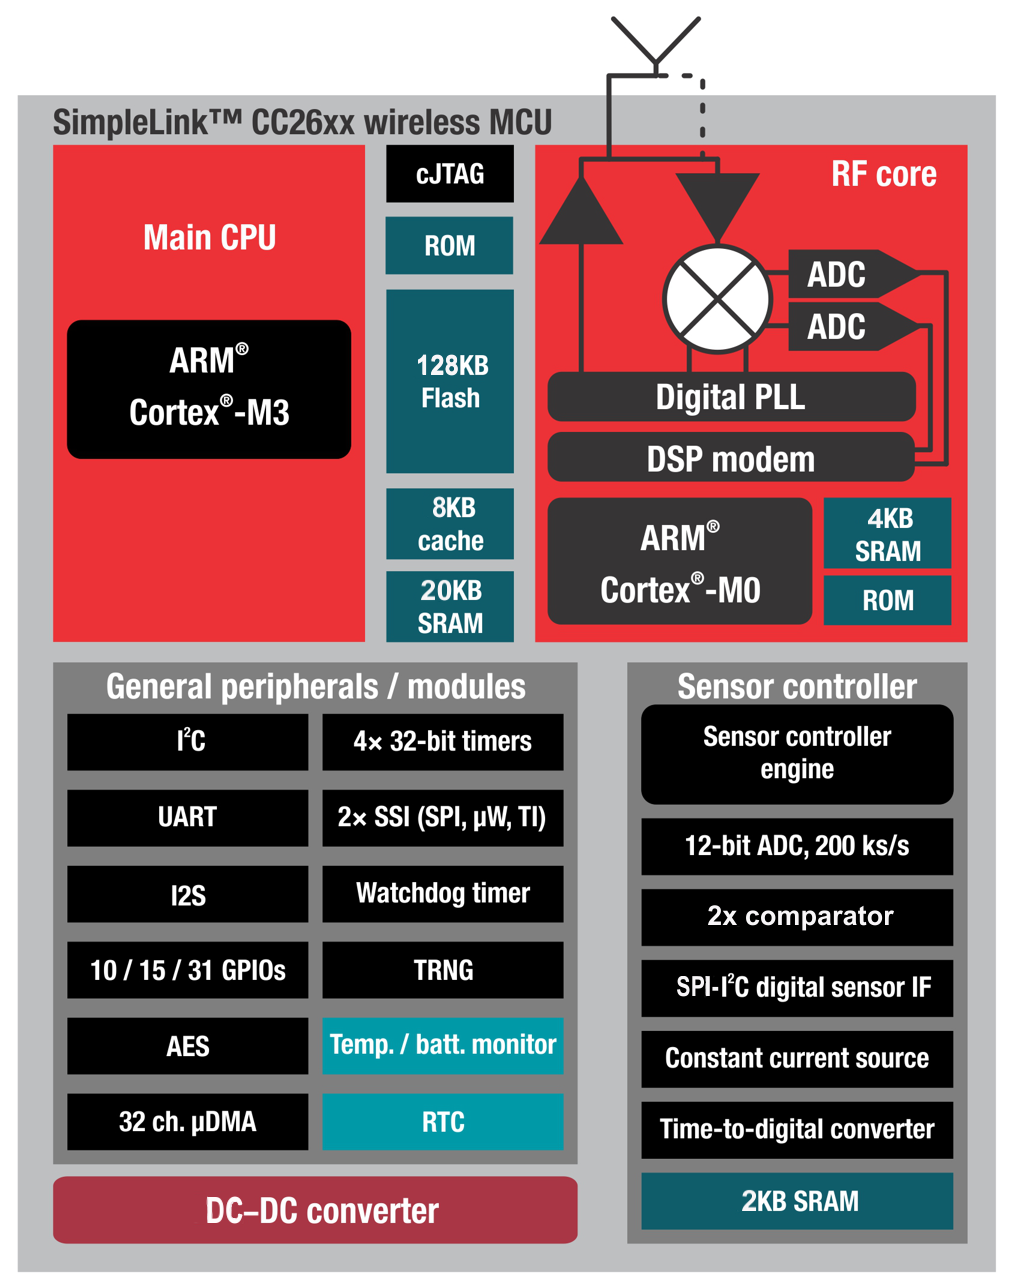
\includegraphics {7Anhang/imag/CC26xx_Block_Diagram.png} 
     \caption{Blockschema Sensortag aus \cite{Sensortag_Datasheet}, S.3}
\end{figure}



\chapter{Messaufbau}
\label{messaufbau}

Um reproduzierbare Werte zu erhalten, wurde eine Radimitation mit einem elektrischen Motor aufgestellt. Die Radimitation besitzt nur eine Speicheimitation. Dies ist eine Alustange, mit mehreren Löchern für das Anbringen des Magneten nach gewünschtem Abstand.

\todo{Bild einfügen}
Bild.

Der Radimitation ist ein Tachometer angehängt, der die aktuelle Geschwindigkeit anzeigt. 

Im Verlauf der Entwicklung wurde entschieden, dass zwei Magnete im Abstand von 180 Grad angebracht werden. Dies, damit genug Energie zur Verfügung steht (siehe Messprotokoll xxxxx). 

\todo{Grad Zeichen einbauen}
\todo{Abstand und Radumfang kontrollieren}
Der Grundabstand ist 25 cm, was einen Radumfang von 2.04 m ergibt. Die ersten Messungen, siehe Anhang \ref{uebersicht_messprotokolle} beziehen sich auf diesen Radumfang. Die Messungen xxx beziehen sich auf einen Radumfang von yyyy.

\chapter{Übersicht Messprotokolle}
\label{uebersicht_messprotokolle}

Aufstellung von Manu
\todo{Messprotokoll Liste}

%\chapter{Messprotokoll Energiegewinnung Harvester}\label{anhang_messprotokoll_energie_harvester} 
%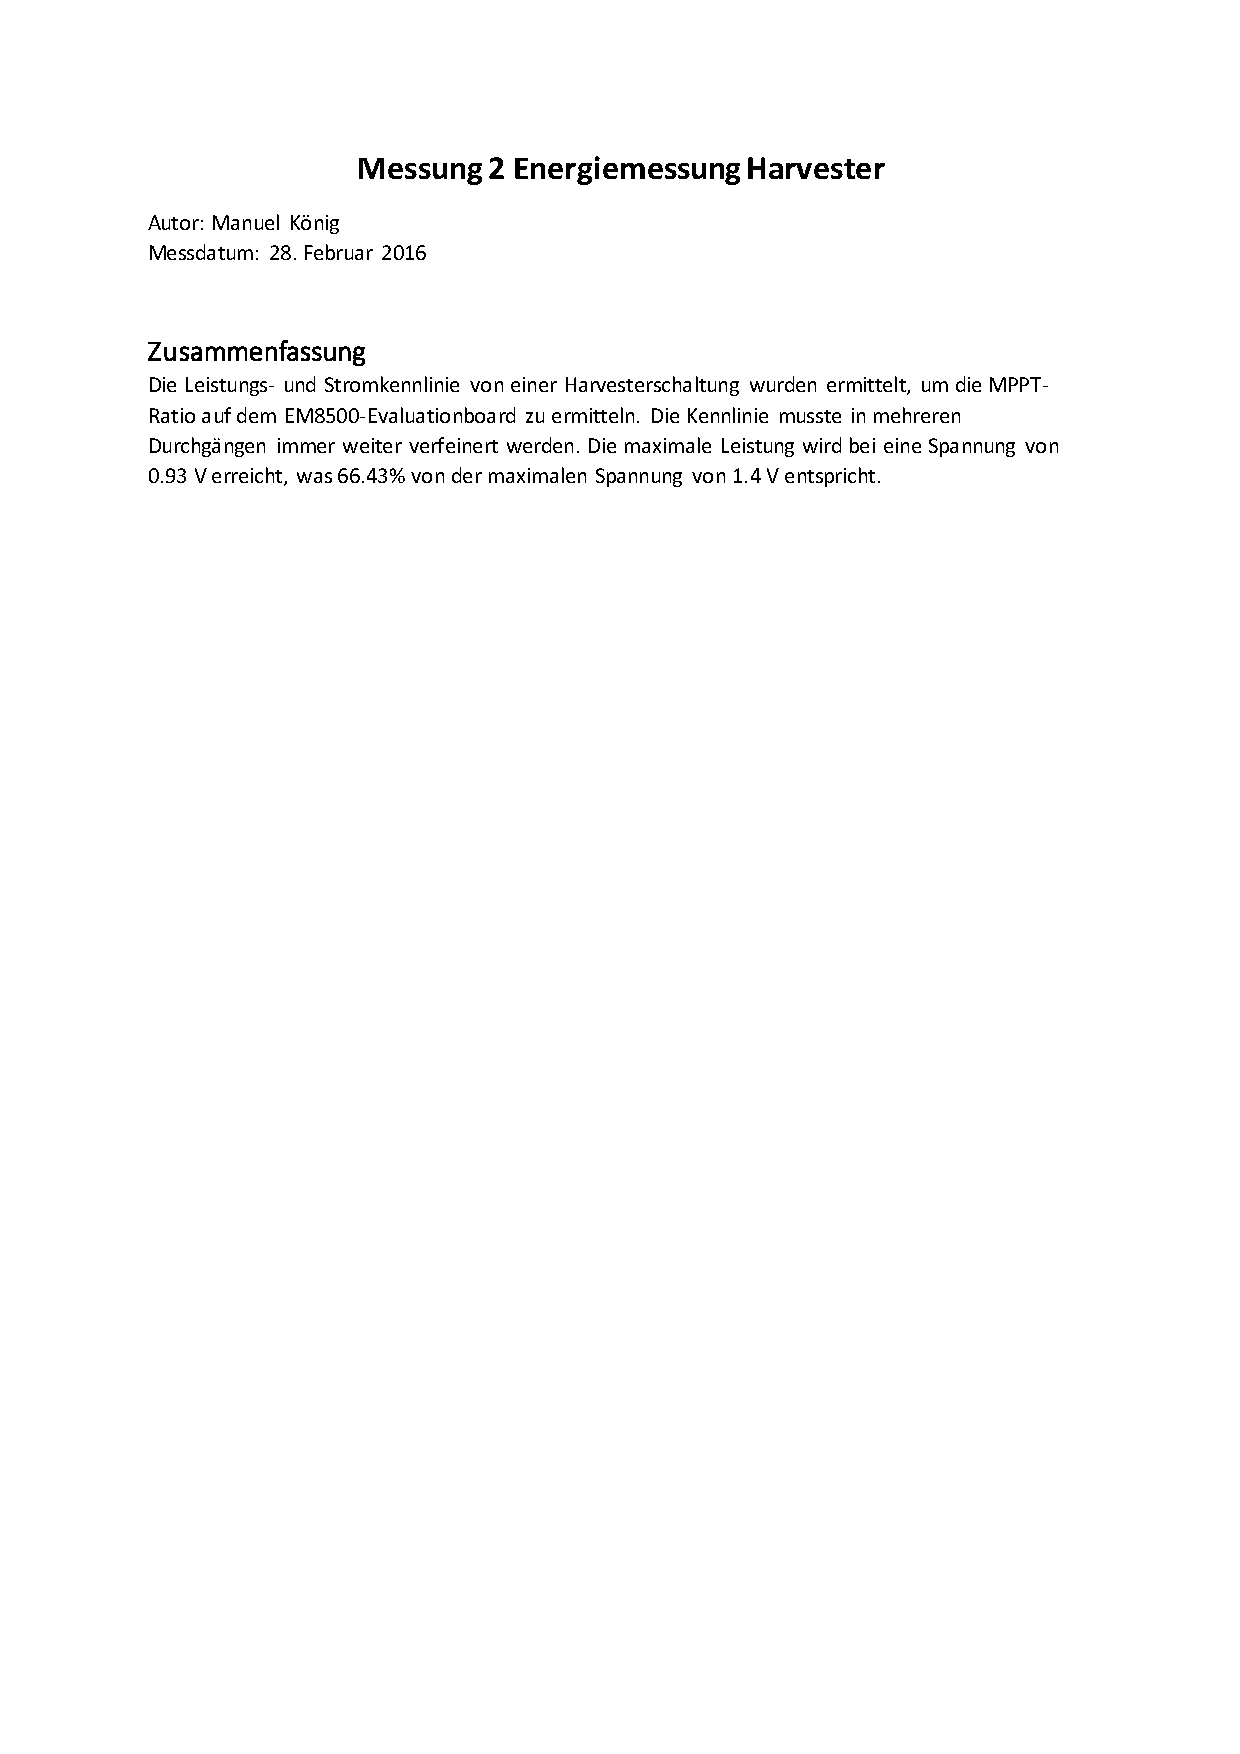
\includepdf[pages=-]{../ressources/Energiemessungen/MessungHarvesterschaltungV0.pdf}
%
%
%\chapter{Messprotokoll Energieverbrauch Sensortag}\label{anhang_messprotokoll_energie_sensortag} 
%%\includepdf{../ressources/Projektorganisation/Ausschreibung.pdf}
%
%\chapter{Messprotokoll Rippelspannung Ausgangskondensator Harvesterschaltung}\label{anhang_messprotokoll_kondensator_harvester} 
%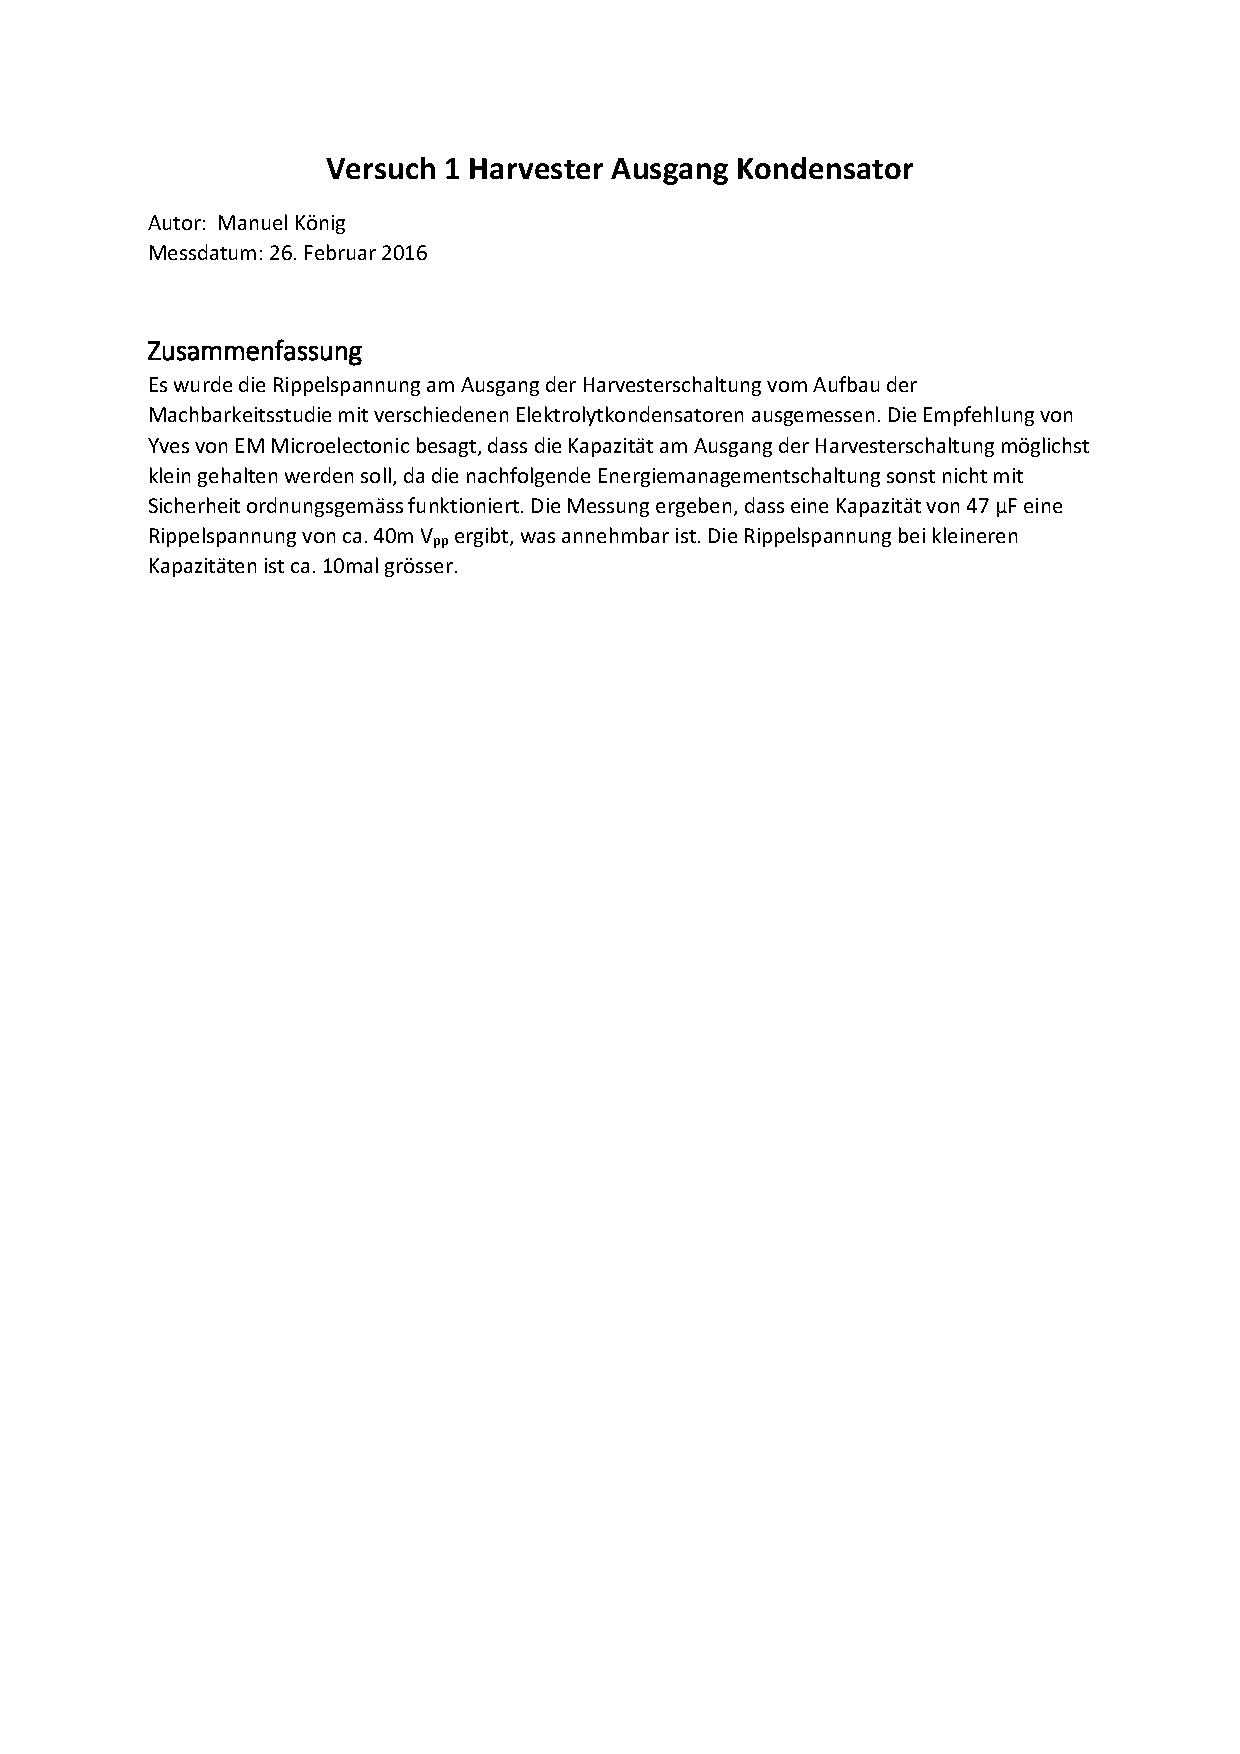
\includepdf[pages=-]{../ressources/Energiemessungen/MessungKondensatorAusgang.pdf}